\chapter{Module assembly}

One option for module assembly is manual assembly with a custom-built mechanical jig (prototype is shown on Figure )

\begin{figure}[ht]\centering
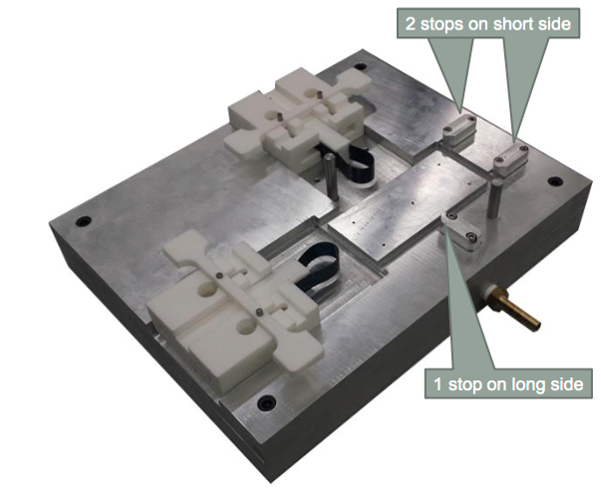
\includegraphics[width=0.8\linewidth]{Data/Module_assembly/Mechanical_jig.png}
\caption{Prototype of the mechanical jig for module assembly}
\label{fig:mechanical jig}
\end{figure}

\section{Automated assembly steps}

[Perhaps I should put this section later...?]
Steps [list]:
1) Spacers to platform
2) Glue upper sensor to spacers
3) Rotate 90 degrees
4) Remove spacer+upper sensor
5) Put baseplate on the assembly platform
6) Glue bottom sensor (bare module) to the baseplate
7) Glue Upper sandwich to the bottom one.


\section{Assembly platform}




\subsection{Requirements for assembly platform}



\subsection{Design}



\section{Fast adhesive}

